\chapter{Analyse der Ergebnisse}
\label{kap:ergebnisse}

Dieses Kapitel wertet die Läufe auf der Instanz aus
Kapitel~\ref{kap:erpolino} aus. Zuerst wird die gefundene Zuordnung
betrachtet, dann die Wirkung der geglätteten Energie, schließlich das
Verhalten beider Verfahren bei wachsender Instanzgröße.

\section{Die gefundene Zuordnung}
\label{sec:zuordnung}

Abbildung~\ref{abb:auslastung} stellt die Auslastung der Mitarbeitenden
für die \ac{lpt}-Startlösung und die Lösung des Verfahrens gegenüber.
Der Unterschied ist weniger die Höhe als die Gleichmäßigkeit: \ac{lpt}
erzeugt ein deutliches Gefälle, das Verfahren zieht die Balken
zusammen. Genau darum geht es -- der \Index{Makespan} ist die Höhe des
höchsten Balkens, alles darunter ist Leerlauf.

\begin{figure}[tb]
  \centering
  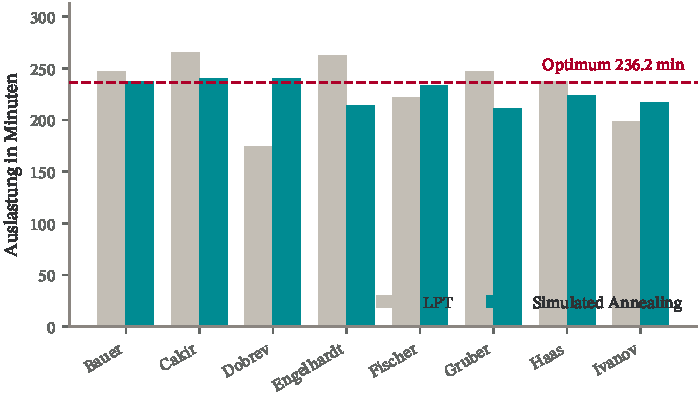
\includegraphics[alt={Gruppiertes Balkendiagramm: Auslastung in Minuten je Mitarbeiterin und Mitarbeiter, jeweils für die LPT-Startlösung und nach Simulated Annealing, dazu eine gestrichelte Linie beim Optimum. Nach Simulated Annealing liegen die Balken gleichmäßiger um das Optimum.}]{Abbildungen/auslastung.pdf}
  \caption[Auslastung je Mitarbeiter]{Auslastung der Mitarbeitenden bei
    der \acs{lpt}-Startlösung und nach dem Verfahren. Der Makespan ist
    die Höhe des jeweils höchsten Balkens.}
  \label{abb:auslastung}
\end{figure}

Auffällig ist, dass selbst die optimale Lösung kein waagerechtes Profil
erzeugt. Die Auslastungen streuen weiterhin um einige Minuten. Das ist
keine Schwäche des Lösers, sondern eine Eigenschaft des Problems:
Aufgaben sind unteilbar, und die Qualifikationen schränken ein, wer was
übernehmen darf. Eine vollkommen gleichmäßige Verteilung ist im
Allgemeinen unzulässig. Sie ist genau die Annahme, auf der die triviale
untere Schranke von \UntereSchranke{} Minuten beruht -- und deshalb
liegt das wahre Optimum mit \Optimum{} Minuten um \LueckeSchranke{}
Prozent darüber.

Wohin die Arbeitszeit fließt, zeigt Abbildung~\ref{abb:sankey}. Die
Bandbreite entspricht den Minuten, die von einer Qualifikation auf einen
Mitarbeitenden entfallen. Sichtbar wird, dass sich die Last der seltenen
Qualifikationen auf wenige Personen konzentriert: Wer als Einziger
schweißen kann, bekommt die Schweißarbeit, unabhängig davon, wie
ausgelastet er ohnehin ist.

\begin{figure}[tb]
  \centering
  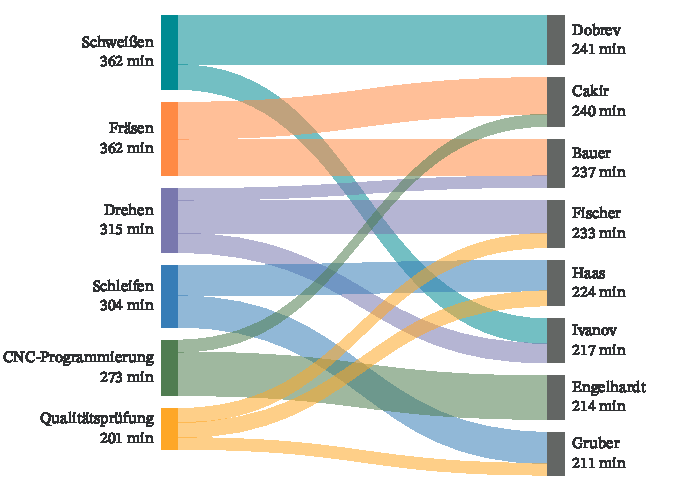
\includegraphics[alt={Flussdiagramm: Bänder führen von den Qualifikationen links zu den Mitarbeitenden rechts; die Breite eines Bandes entspricht den zugeordneten Minuten.}]{Abbildungen/sankey.pdf}
  \caption[Fluss der Arbeitszeit]{Fluss der Arbeitszeit von den
    Qualifikationen zu den Mitarbeitenden in der gefundenen Lösung. Die
    Bandbreite entspricht den Minuten.}
  \label{abb:sankey}
\end{figure}

\section{Wirkung der geglätteten Energie}
\label{sec:energiewirkung}

Abschnitt~\ref{sec:plateau} hat die geglättete Energie mit dem
Plateauproblem begründet. Ob das Argument trägt, ist eine empirische
Frage. Abbildung~\ref{abb:energien} beantwortet sie über je 20~Läufe
beider Varianten.

\begin{figure}[tb]
  \centering
  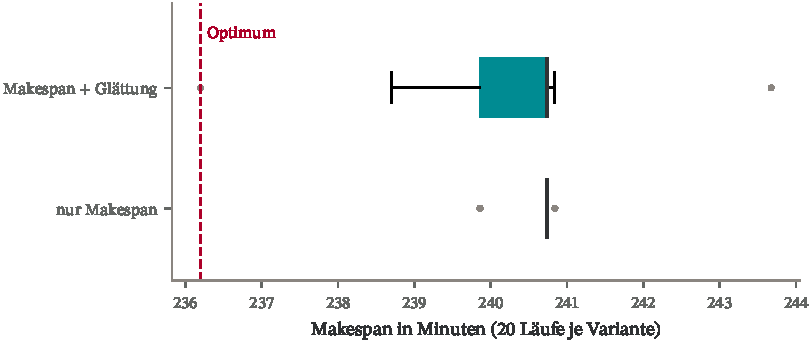
\includegraphics[alt={Kastendiagramme des Makespans über mehrere Läufe für zwei Energiefunktionen, dazu eine gestrichelte Linie beim Optimum. Nur mit Glättungsterm erreicht ein Lauf das Optimum.}]{Abbildungen/energien.pdf}
  \caption[Wirkung der geglätteten Energie]{Streuung des Makespans über
    je 20 Läufe. Mit der rohen Zielgröße als Energie erreicht kein Lauf
    das Optimum; mit dem Glättungsterm gelingt es.}
  \label{abb:energien}
\end{figure}

Der Befund ist deutlich. Mit der rohen Zielgröße liegen alle Läufe eng
beieinander bei \SaRohMittel{} Minuten im Mittel -- eng, aber
gleichmäßig zu hoch. Das Verfahren findet zuverlässig dasselbe lokale
Optimum und kommt nicht darüber hinaus. Mit dem Glättungsterm sinkt der
Mittelwert auf \SaMittel{} Minuten, und der beste Lauf erreicht mit
\SaBestes{} Minuten das Optimum.

Bemerkenswert ist der Preis: Die Streuung nimmt zu. Die geglättete
Variante ist im Mittel besser, aber weniger vorhersagbar. Wer einen
einzelnen Lauf betrachtet, kann schlechter abschneiden als mit der rohen
Variante. Das ist der übliche Handel zwischen Erkundung und
Verlässlichkeit und ein Argument dafür, mehrere Läufe zu rechnen und den
besten zu nehmen -- was bei einer Rechenzeit von \SaMillisekunden{}
Millisekunden je Lauf keine ernsthafte Hürde ist.

Abbildung~\ref{abb:konvergenz} zeigt einen einzelnen Lauf im Verlauf.
Die aktuelle Lösung schwankt anfangs stark -- die Temperatur lässt
Verschlechterungen zu --, und beruhigt sich mit sinkender Temperatur.
Die beste gefundene Lösung fällt in Stufen: lange Phasen ohne
Fortschritt, unterbrochen von Sprüngen. Genau dieses Muster erwartet man
bei einer plateaulastigen Zielgröße.

\begin{figure}[tb]
  \centering
  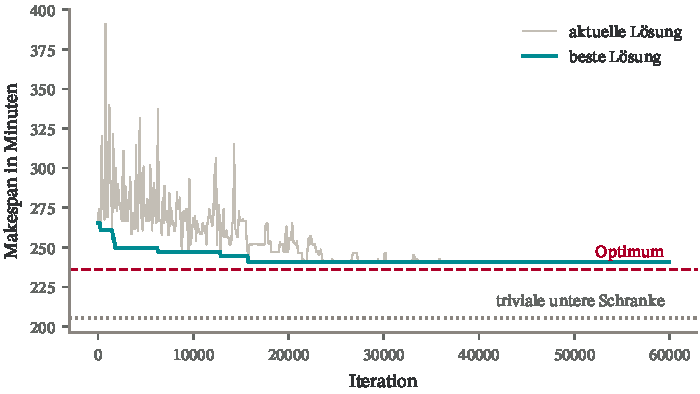
\includegraphics[alt={Liniendiagramm über die Iterationen: aktuelle und beste Lösung fallen ab und nähern sich der Linie des Optimums; darunter die untere Schranke.}]{Abbildungen/konvergenz.pdf}
  \caption[Verlauf eines Laufs]{Verlauf eines einzelnen Laufs: aktuelle
    und beste Lösung, dazu Optimum und triviale untere Schranke.}
  \label{abb:konvergenz}
\end{figure}

\section{Vergleich der Verfahren}
\label{sec:vergleich}

Tabelle~\ref{tab:verfahren} auf Seite~\pageref{tab:verfahren} hat die
Verfahren bereits gegenübergestellt. Die Rangfolge ist eindeutig: Die
bisherige Praxis entspricht ungefähr der Greedy-Regel mit
\MakespanGreedy{} Minuten, \ac{lpt} verbessert das auf \MakespanLPT{}
Minuten, \ac{sa} auf \MakespanSA{} Minuten, und das exakte Verfahren
erreicht \Optimum{} Minuten.

Gegenüber der heutigen Praxis spart die optimale Lösung rund eine halbe
Stunde je Fertigungslos. Das ist der Ertrag, um den es geht, und er ist
mit einem Standardlöser in weniger als einer Sekunde zu haben.

Damit stellt sich die Frage nach dem Sinn der Heuristik in aller
Schärfe. Auf dieser Instanz ist \ac{sa} in jeder Hinsicht unterlegen: Es
braucht mehr Rechenzeit als der exakte Löser, findet ein um
\AbstandSA{} Prozent schlechteres Ergebnis und gibt keinerlei Garantie.
Wer nur diese Instanz betrachtet, sollte den Löser nehmen.

\section{Verhalten bei wachsender Instanz}
\label{sec:skalierung}

Der Vorteil des exakten Verfahrens ist allerdings an die Größe gebunden.
Um zu prüfen, wo die Grenze liegt, wurden Zufallsinstanzen derselben
Struktur mit wachsender Zahl von Arbeitsgängen erzeugt und beide
Verfahren darauf angewendet. Dem Löser wurde eine Zeitschranke von
30~Sekunden gesetzt.

\begin{table}[tb]
  \centering
  % Automatisch erzeugt von Code/tabellen.py -- nicht von Hand ändern.
% Quelle: Code/daten.py und Ergebnisse/*.json

\begin{tabular}{@{}S[table-format=3.0]S[table-format=2.0]S[table-format=3.2]S[table-format=2.1]lS[table-format=3.2]S[table-format=1.1]S[table-format=+1.2]@{}}
\toprule
& & \multicolumn{3}{c}{MILP (GLPK)} & \multicolumn{2}{c}{Simulated Annealing} & \\
\cmidrule(lr){3-5}\cmidrule(lr){6-7}
{Aufg.} & {Mitarb.} & {Makespan} & {Zeit} & {Status} & {Makespan} & {Zeit} & {Abstand} \\
& & {min} & {s} & & {min} & {s} & {\%} \\
\midrule
  24 & 8 & 276.77 & 1.1 & optimal & 280.80 & 0.3 & +1.46 \\
  40 & 10 & 381.45 & 0.0 & optimal & 381.45 & 0.4 & +0.00 \\
  60 & 12 & 529.71 & 30.0 & Zeitschranke & 529.33 & 0.5 & -0.07 \\
  80 & 14 & 489.17 & 30.0 & Zeitschranke & 484.03 & 0.7 & -1.05 \\
  120 & 18 & 707.27 & 30.0 & Zeitschranke & 707.27 & 1.0 & +0.00 \\
\bottomrule
\end{tabular}

  \caption[Verhalten bei wachsender Instanz]{Beide Verfahren auf
    Zufallsinstanzen wachsender Größe. Ein negativer Abstand bedeutet,
    dass Simulated Annealing die beste Lösung schlägt, die der Löser
    innerhalb der Zeitschranke gefunden hat.}
  \label{tab:skalierung}
\end{table}

\begin{figure}[tb]
  \centering
  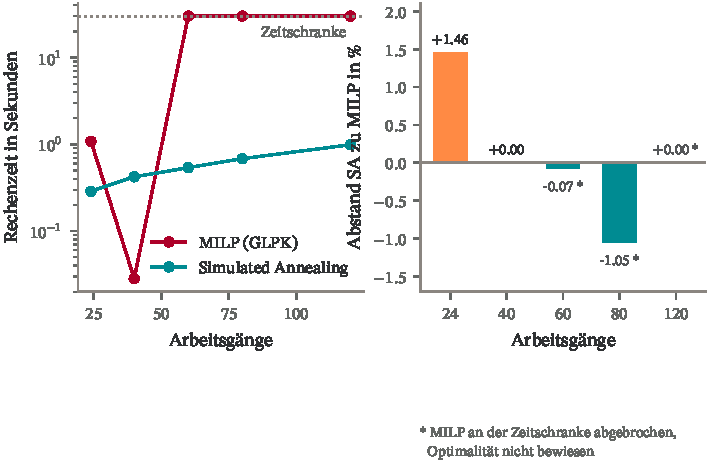
\includegraphics[alt={Links: Rechenzeit von MILP und Simulated Annealing über der Zahl der Arbeitsgänge, logarithmisch; das MILP stößt ab mittlerer Größe an die Zeitschranke. Rechts: Balken mit dem prozentualen Abstand von Simulated Annealing zum MILP je Instanzgröße.}]{Abbildungen/skalierung.pdf}
  \caption[Rechenzeit und Güte über die Instanzgröße]{Rechenzeit
    (links, logarithmisch) und Abstand der Lösungen (rechts) über die
    Zahl der Arbeitsgänge.}
  \label{abb:skalierung}
\end{figure}

Tabelle~\ref{tab:skalierung} und Abbildung~\ref{abb:skalierung} zeigen
den Umschlag. Bis 40~Arbeitsgänge löst \ac{glpk} beweisbar optimal,
teilweise in Sekundenbruchteilen. Ab 60~Arbeitsgängen läuft der Löser in
die Zeitschranke und kann die Optimalität nicht mehr belegen. Von da an
liefert \ac{sa} in unter einer Sekunde Lösungen, die gleich gut oder
besser sind als das, was der Löser in 30~Sekunden erreicht -- bei
80~Arbeitsgängen um gut ein Prozent besser.

Zwei Beobachtungen verdienen Beachtung. Erstens verläuft die Rechenzeit
des Lösers nicht monoton: Die Instanz mit 40~Arbeitsgängen ist leichter
als die mit 24. Die Schwierigkeit einer Instanz hängt eben nicht allein
an ihrer Größe, sondern an ihrer Struktur -- eine bekannte, aber gern
übersehene Eigenschaft ganzzahliger Probleme. Zweitens wächst die
Rechenzeit von \ac{sa} nur schwach, weil sie durch die feste Zahl von
Iterationen bestimmt ist und nicht durch die Instanz. Das macht sie
planbar, sagt aber nichts über die Güte.

\section{Grenzen der Aussage}

Die Ergebnisse dieses Kapitels gelten für die untersuchte Instanz und
die untersuchten Zufallsinstanzen. Fünf Größen mit je einer Instanz sind
eine schmale Grundlage; belastbar wäre eine Auswertung über mehrere
Instanzen je Größe mit Angabe der Streuung. Ebenso wurde nur ein Löser
betrachtet. Kommerzielle Löser sind auf ganzzahligen Problemen
regelmäßig um Größenordnungen schneller als \ac{glpk}, was den
Umschlagpunkt nach oben verschieben dürfte -- vermutlich deutlich.

Die Aussage \enquote{ab etwa 60~Arbeitsgängen lohnt sich die Heuristik}
ist deshalb genauer zu lesen als: \enquote{mit diesem Löser, dieser
Zeitschranke und dieser Instanzstruktur}. Die Struktur des Arguments
bleibt gültig, die Zahl ist keine Konstante.
